\begin{egBox}{Example of a Basis in \( \mathbb{R}^{ 2 } \)}[eg:13-1]
    Let \( X = \mathbb{R}^{ 2 } \). 
    Let \( \mathcal{B} \) be the collection of all balls in the plane.
    Then \( \mathcal{B} \) satisfies both conditions of a basis;
    indeed, the first condition is met as we can always put a ball around 
    any \( x \in X \), and the second condition is illustrated in 
    Figure \ref{fig:13-2}

    \begin{figure}[H]
        \centering
        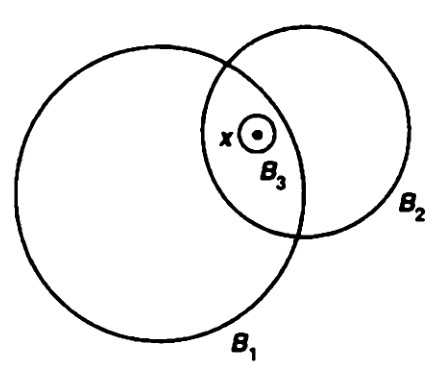
\includegraphics[ width = 0.3\linewidth ]{figures/Section 13/basis2.jpg}
        \caption{A Visual of the Second Condition}
        \label{fig:13-2}
    \end{figure}

    In the topology generated by \( \mathcal{B} \), we also have that the 
    definition of openness can be rewritten as follows: a subset \( U \) of the 
    plane is open if every \( x \in U \) lies within some ball contained
    in \( U \) -- this is the definition of openness that we learned in the 
    metric spaces section earlier on.
\end{egBox}

\begin{egBox}{Another Example of a Basis in \( \mathbb{R}^{ 2 } \)}[eg:13-2]
    Let \( X = \mathbb{R}^{ 2 } \). 
    Let \( \mathcal{B}' \) be the collection of all rectangular regions 
    (interiors of rectangles) in the plane, where the rectangles have sides 
    parallel to the coordinate axes.
    Then \( \mathcal{B}' \) satisfies both conditions of a basis;
    indeed, the first condition is met as we can always put a rectangular
    region around any \( x \in X \), and the second condition is illustrated in 
    Figure \ref{fig:13-3}

    \begin{figure}[H]
        \centering
        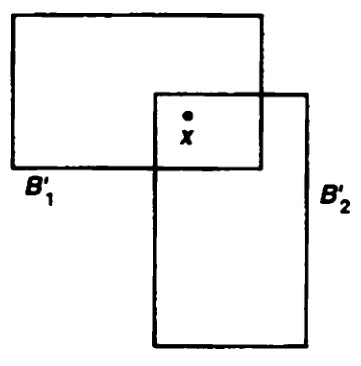
\includegraphics[ width = 0.3\linewidth ]{figures/Section 13/basis3.jpg}
        \caption{A Visual of the Second Condition}
        \label{fig:13-3}
    \end{figure}

    One can see that the second condition is trivial since the intersection of 
    any two basis elements is either another rectangular region (hence, a basis 
    element) or the empty set.

    \baseSkip 

    In fact, we have that the basis \( \mathcal{B} \) from the previous example
    generates the same topology as the collection \( \mathcal{B}' \) of 
    all rectangular regions. Figure \ref{fig:13-4} illustrates the proof.

    \begin{figure}[H]
        \centering
        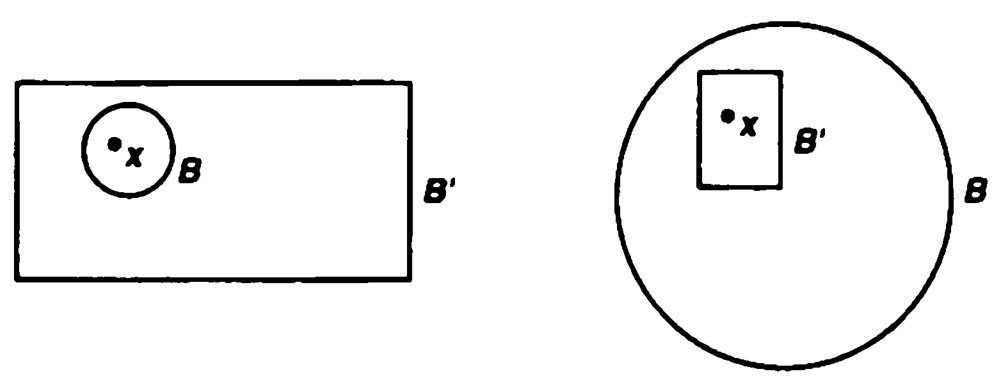
\includegraphics[ width = 0.6\linewidth ]{figures/Section 13/basis4.jpg}
        \caption{A Visual Proof}
        \label{fig:13-4}
    \end{figure}
\end{egBox}

\begin{egBox}{Basis for a Discrete Topology}[eg:13-4]
    If \( X \) is any set, then the collection of all one-point subsets of 
    \( X \) is a basis for the discrete topology on \( X \).

    \baseSkip 

    The first condition of a basis is met trivially -- for any \( x \in X \),
    it is contained in the one-point subset \( \{ x \} \). 
    For the second condition, we have that \( x \) will only belong to one 
    one-point subset -- i.e., the intersection of any two one-point subsets 
    is \( \emptyset \). Thus, the second condition is vacuously met (there is 
    nothing to check!).
\end{egBox}

\begin{egBox}{Basis for \( \mathbb{R}_{ \ell } \)}[eg:13-5]
    We want to show that the collection of all half-open intervals of the 
    form 
    \begin{equation*}
        [ a, b )
        =
        \{ x \mid a \leq x < b \}
    \end{equation*} 
    where \( a < b \), is indeed a basis of \( \mathbb{R} \).

    \baseSkip

    For the first condition (fullness), we let \( x \in \mathbb{R} \). 
    It is clear to see that \( x \in [ x, x + 1 ) \), but there are many more 
    other possibilities.

    \baseSkip 

    For the second condition (smallness), we let 
    \( x \in [ a, b ) \cap [ c, d ) \), where \( a < c \), WLOG.
    We shall focus on the case when \( b < d \) to save some time.
    Notice that if the intersection is not \( \emptyset \), then we get 
    \( [ a, b ) \cap [ c, d ) = [ c, b ) \).
    Thus, we have \( x \in [ c, b ) \), which fulfills the smallness condition. 
    If we have \( \emptyset \) instead, then we see that the smallness 
    condition is met vacuously.
\end{egBox}

\begin{egBox}{Topology Generated by a Basis Verification}[eg:13-6]
    We want to show that the collection \( \mathcal{T} \) generated by the basis \( \mathcal{B} \) is indeed a topology on 
    \( X \).  
    
    \baseSkip 
    \wrapBox{\( \emptyset, X \in \mathcal{T} \)}
    \baseSkip

    For this condition, we need to check that both \( \emptyset \) and \( X \) 
    are open. 
    We start by noting that \( \emptyset \) satisfies the defining conditions 
    of openness vacuously (there is nothing to check since \( \emptyset \) has 
    no elements).
    
    \baseSkip

    Now to show that \( X \) is open, we need to show that for each 
    \( x \in X \), there is a basis element \( B \in \mathcal{B} \) 
    such that \( x \in B \) and \( B \subset X \). 
    This immediately follows from the fact that we have a basis 
    \( \mathcal{B} \) -- by definition, each basis element is a subset of 
    \( X \), and for each \( x \in X \), there is at least one basis element 
    \( B \) containing \( x \).

    \baseSkip 
    \wrapBox{\( \mathcal{T} \) is closed under unions}
    \baseSkip

    For this condition, let us take an indexed family 
    \( \{ U_{ i } \}_{ i \in I } \), of elements of \( \mathcal{T} \). 
    We want to show that \( \mathcal{T} \) is closed under unions -- 
    that is, we want to show that 
    \begin{equation*}
        U = \bigcup_{ i \in I } U_{ i }
    \end{equation*}
    belongs to \( \mathcal{T} \). 
    To do so, we need to check that \( U \) is open. 
    
    \baseSkip
    
    Let's say that we are given some \( x \in U \). 
    It follows that there is at least one index \( i \) such that 
    \( x \in U_{ i } \). 
    Since we know that \( U_{ i } \in \mathcal{T} \), it follows that 
    \( U_{ i } \) is open, which further means (by the definition of 
    openness via a basis) that there exists some basis element 
    \( B \in \mathcal{B} \) such that \( x \in B \) and \( B \subset U_{ i } 
    \subset U \). 
    Hence, it follows that \( U \) is open.

    \baseSkip 
    \wrapBox{\( \mathcal{T} \) is closed under finite intersections}
    \baseSkip

    For this condition, we want to show that \( \mathcal{T} \) is closed under 
    finite intersections. 
    If we have \( n \) elements \( U_{ 1 }, \ldots, U_{ n } \) of 
    \( \mathcal{T} \), then all we need to do is to show that 
    \( U_{ 1 } \cap \ldots \cap U_{ n } \in \mathcal{T} \), 
    which requires us to check that 
    \( U_{ 1 } \cap \ldots \cap U_{ n } \) is open. 
    We shall do so via induction.

    \baseSkip 

    For \( n = 1 \), we are done since \( U_{ 1 } \in \mathcal{T} \) by construction. 
    Let us check for \( n = 2 \).
    Our goal is to show that \( U_{ 1 } \cap U_{ 2 } \in \mathcal{T} \). 
    Given \( x \in U_{ 1 } \cap U_{ 2 } \), we can choose basis elements 
    \( B_{ 1 }, B_{ 2 } \) such that \( x \in B_{ 1 } \), \( x \in B_{ 2 } \) 
    and \( B_{ 1 } \subset U_{ 1 } \), \( B_{ 2 } \subset U_{ 2 } \) since we 
    know both \( U_{ 1 } \) and \( U_{ 2 } \) to be open. 
    Now because we are given a basis, we have its second condition enables us 
    to choose a basis element \( B_{ 3 } \) containing \( x \) such that 
    \( B_{ 3 } \subset B_{ 1 } \cap B_{ 2 } \). A visual of this condition is
    shown in Figure \ref{fig:13-1}
    
    \begin{figure}[H]
        \centering
        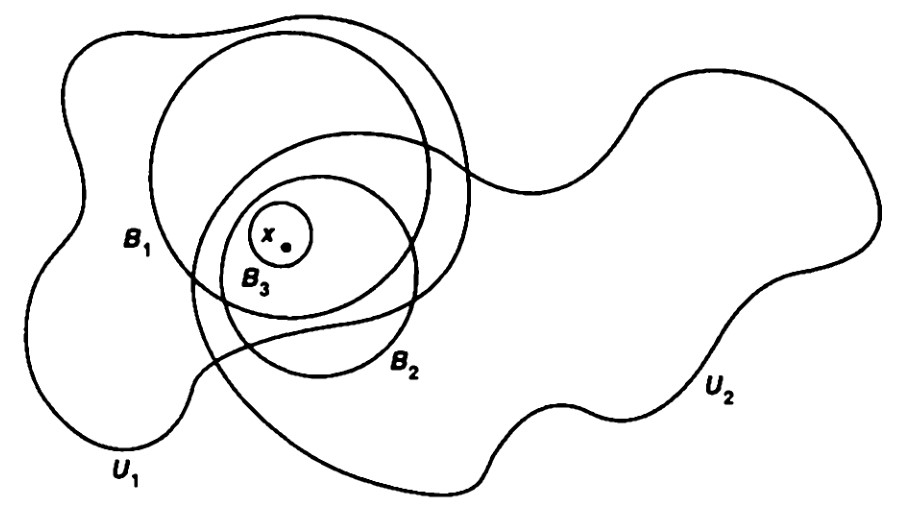
\includegraphics[ width = 0.6\linewidth ]{figures/Section 13/basis1.jpg}
        \caption{A Visual on the Second Condition}
        \label{fig:13-1}
    \end{figure}
    
    Thus, we have that 
    \( x \in B_{ 3 } \) and \( B_{ 3 } \subset U_{ 1 } \cap U_{ 2 } \), which 
    tells us that \( U_{ 1 } \cap U_{ 2 } \) is open -- that is, we have 
    \( U_{ 1 } \cap U_{ 2 } \in \mathcal{T} \). 

    \baseSkip

    Finally, we suppose that it is true for \( n - 1 \) and prove it for
    \( n \). Notice that 
    \begin{equation*}
        U_{ 1 } \cap \ldots \cap U_{ n }
        =
        ( U_{ 1 } \cap \ldots \cap U_{ n - 1 } ) \cap U_{ n }
    \end{equation*}
    By our induction hypothesis, we have that 
    \( U_{ 1 } \cap \ldots \cap U_{ n - 1 } \in \mathcal{T} \). 
    Further notice that this reduces us down to the \( n = 2 \) case, which 
    we have already solved for. Thus, we have the intersection of 
    \( U_{ 1 } \cap \ldots \cap U_{ n - 1 } \) and \( U_{ n } \) also belongs 
    to \( \mathcal{T} \). 
    
    \baseSkip

    Thus, we have checked that the collection of open sets generated by a 
    basis \( \mathcal{B} \) is a topology. 
\end{egBox}

\begin{egBox}{Subbasis Topology Verification}[eg:13-7]
    It suffices to show that the collection \( \mathcal{B} \) of all finite 
    intersections of elements of \( \mathcal{S} \) is a basis. 
    By doing so, [\hyperlink{lem:13.1}{Lemma 1}] tells us that the collection 
    \( \mathcal{T} \) of all unions of elements of \( \mathcal{B} \) is a 
    topology.

    \baseSkip

    We start with the first condition for a basis.
    For any given \( x \in X \), we have that it belongs to some element of 
    \( \mathcal{S} \), and hence, to an element of \( \mathcal{B} \).

    \baseSkip 

    For the second condition, we let 
    \begin{equation*}
        B_{ 1 } 
        =
        S_{ 1 } \cap \ldots \cap S_{ m }
        \quad \mathrm{and} \quad
        B_{ 2 }
        =
        S_{ 1 }' \cap \ldots \cap S_{ n }'
    \end{equation*}
    be two elements of \( \mathcal{B} \). 
    We now let 
    \begin{equation*}
        B_{ 3 } 
        =
        B_{ 1 } \cap B_{ 2 }
        =
        ( S_{ 1 } \cap \ldots \cap S_{ m } )
        \cap 
        ( S_{ 1 }' \cap \ldots \cap S_{ n }' )
    \end{equation*}
    which we also see to be a finite intersection of elements of 
    \( \mathcal{S} \), so we have that \( B_{ 3 } \in \mathcal{B} \).
    Since \( B_{ 3 } = B_{ 1 } \cap B_{ 2 } \), it is also the case that 
    \( B_{ 3 } \subset B_{ 1 } \cap B_{ 2 } \), which satisfies the 
    second condition.
\end{egBox}